\documentclass[landscape,twocolumn]{article}
\usepackage{graphicx}
\usepackage{caption}
\usepackage{lipsum} % for generating dummy text
\usepackage{lscape} % for landscape orientation

% Set default path for images
\graphicspath{{../blender_color/}} % Adjust the path as needed

\DeclareCaptionLabelFormat{step}{Step #2}
\captionsetup[figure]{labelformat=step}

\begin{document}

% \begin{landscape}
\pagestyle{empty} % Remove page numbers

\begin{figure}[p]
    \centering
    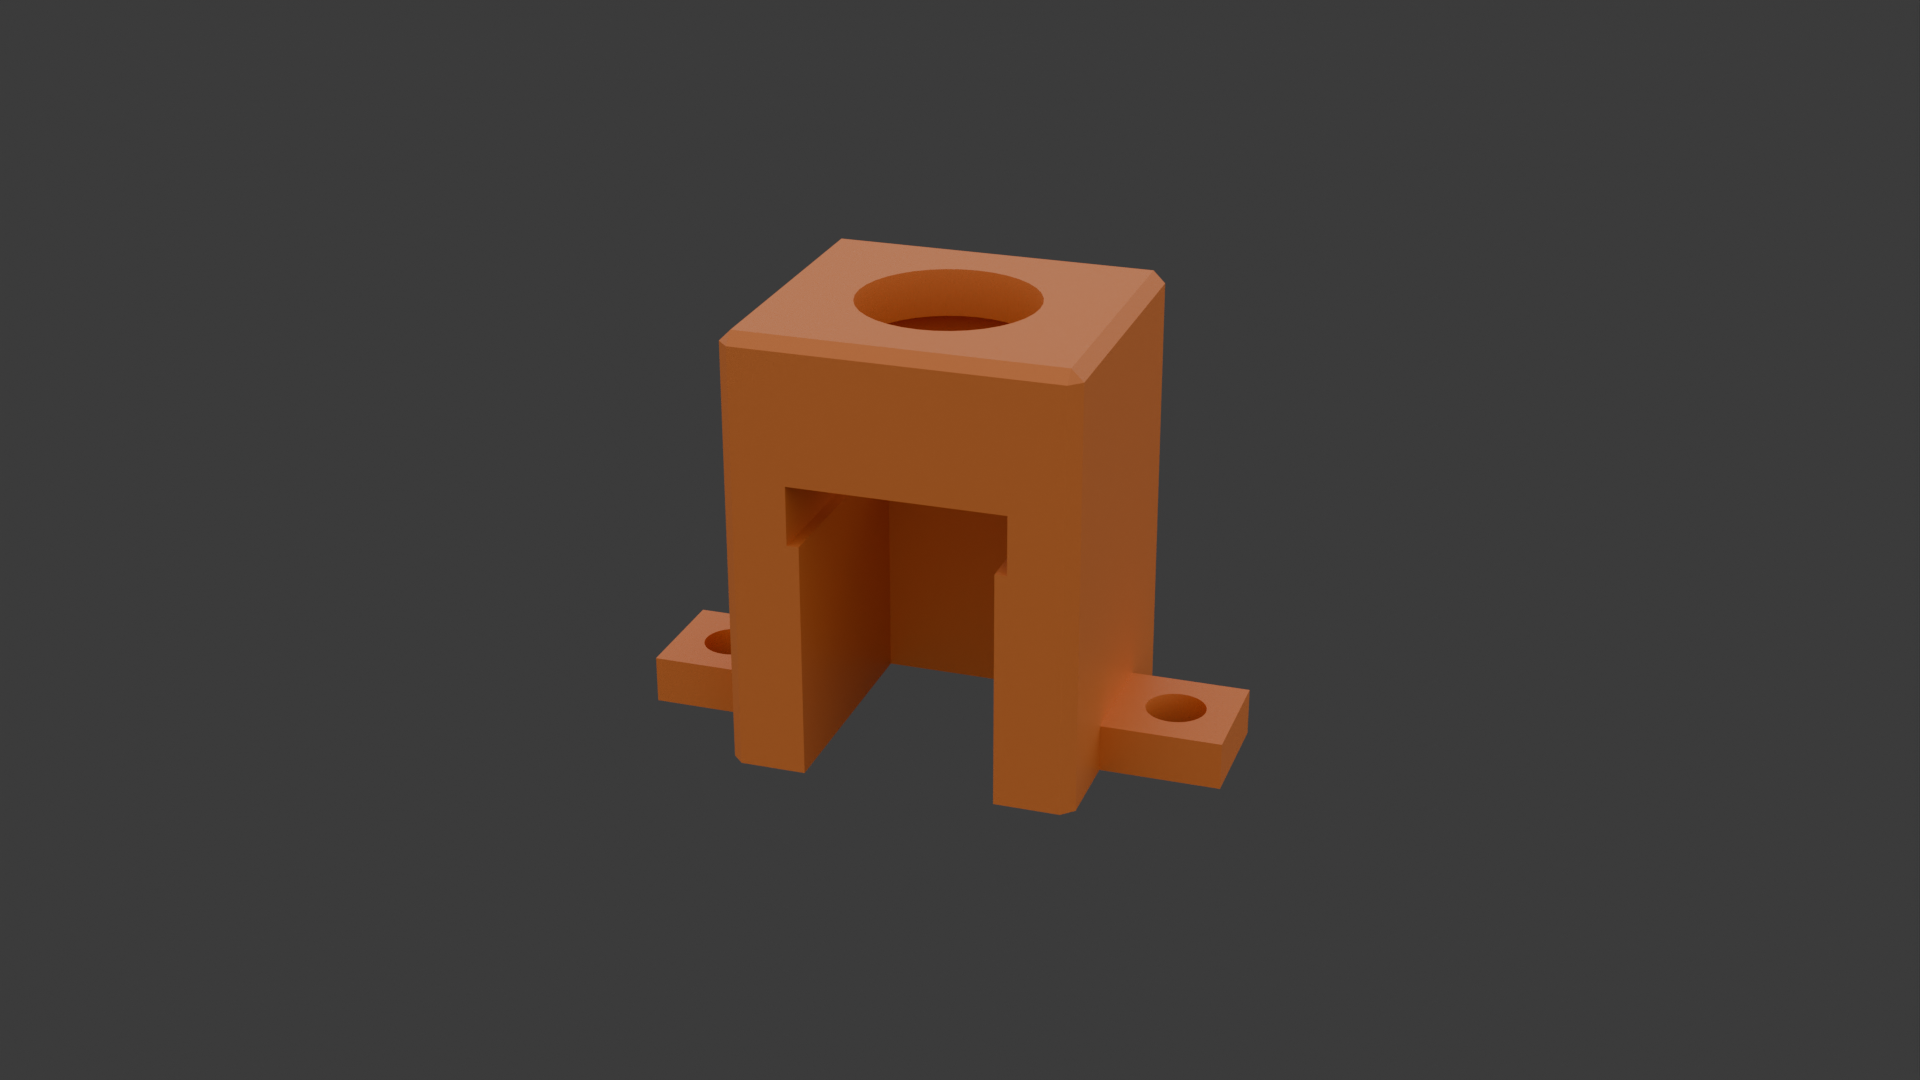
\includegraphics[width=0.875\linewidth]{a.png} % Replace with your image file name
    \caption{Caption for the image}
\end{figure}

% \clearpage

\begin{figure}[p]
    \centering
    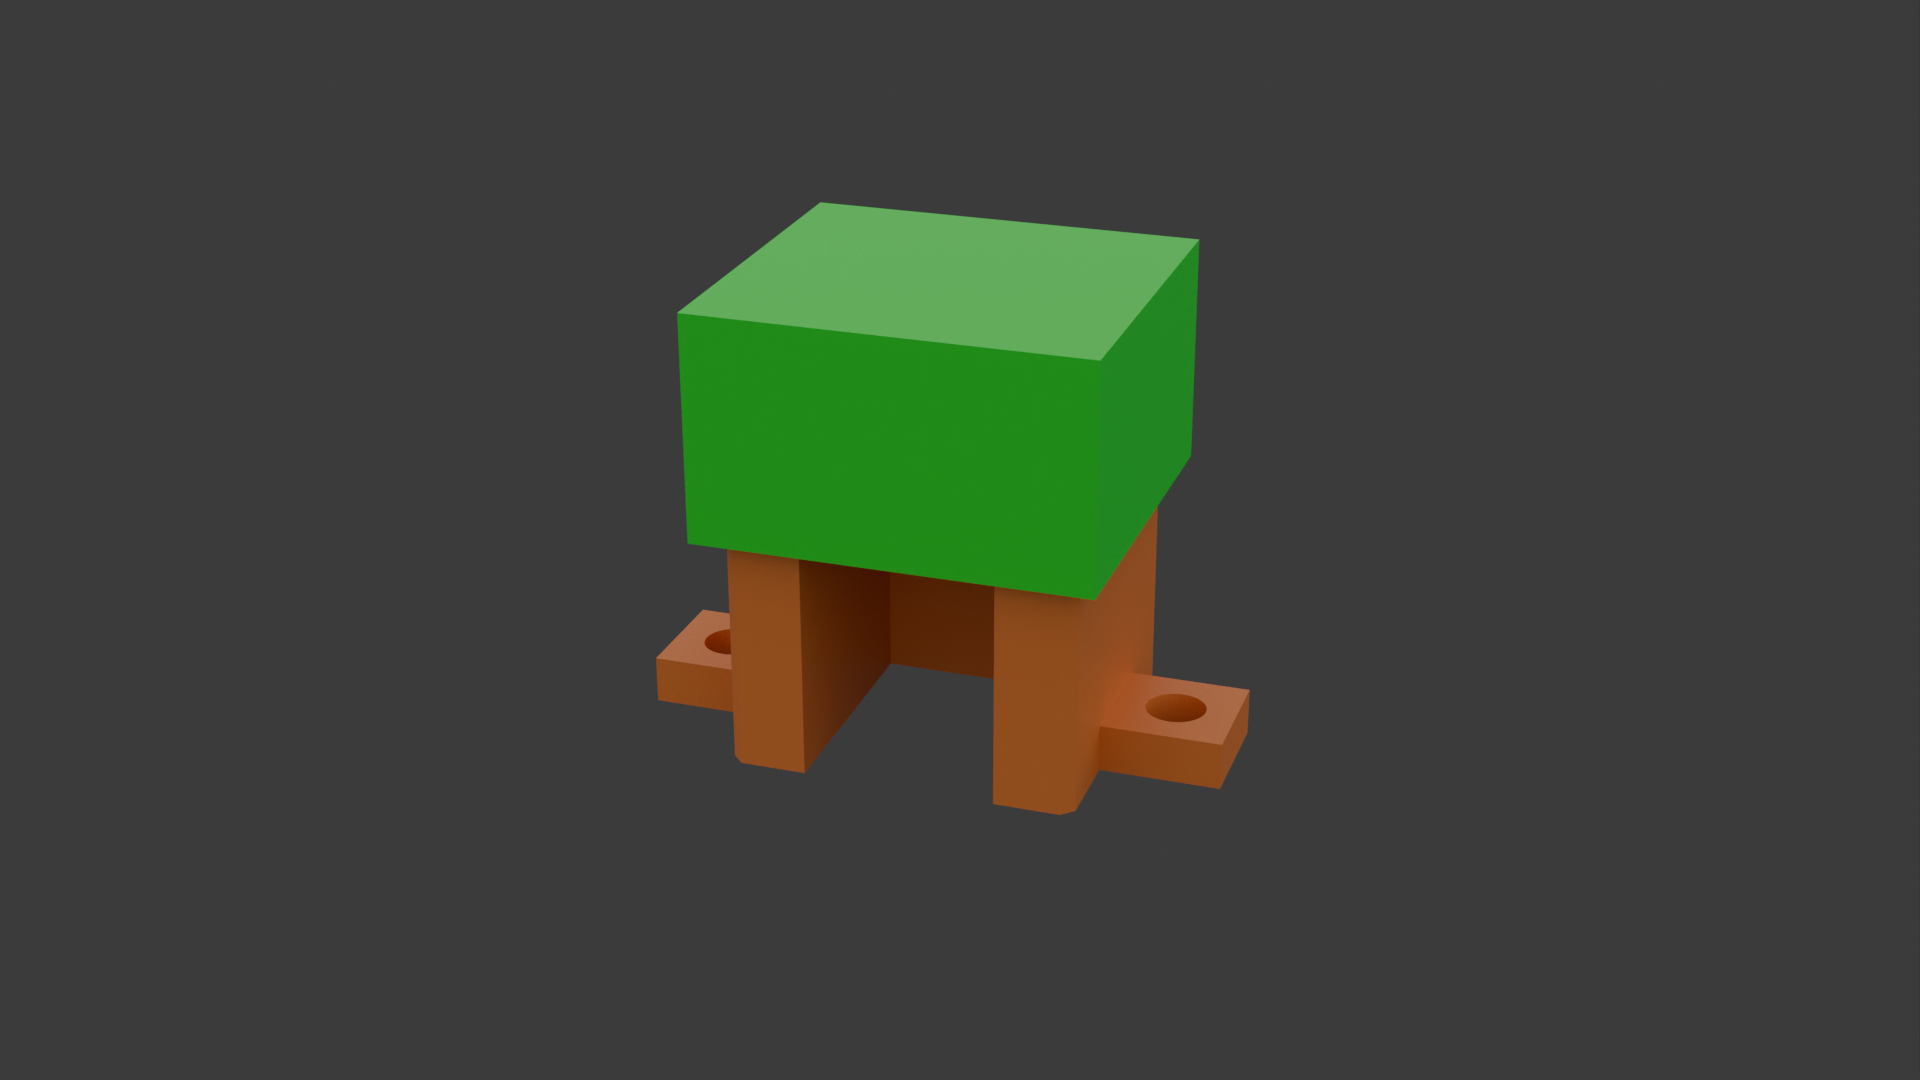
\includegraphics[width=0.875\linewidth]{b.png} % Replace with your image file name
    \caption{Caption for the image}
\end{figure}

% \clearpage

\begin{figure}[p]
    \centering
    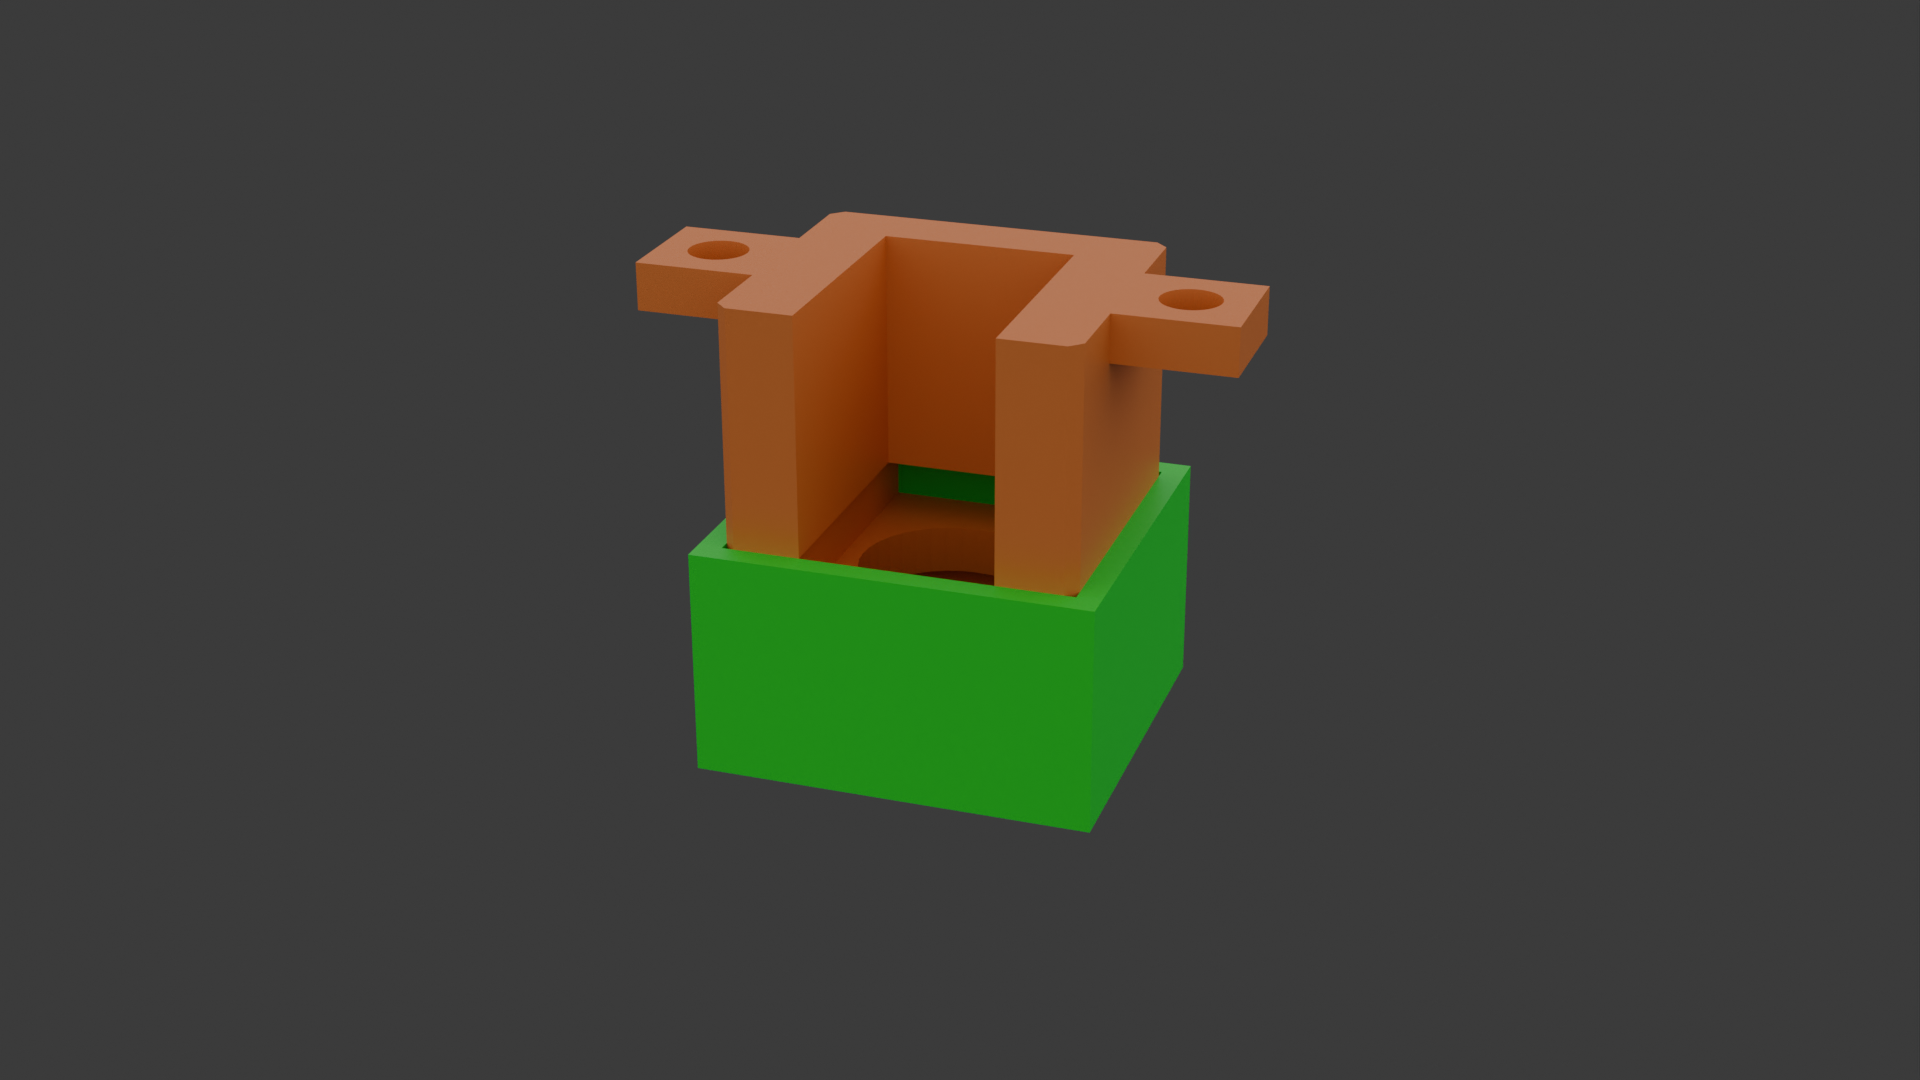
\includegraphics[width=0.875\linewidth]{c.png} % Replace with your image file name
    \caption{Caption for the image}
\end{figure}

% \clearpage

\begin{figure}[p]
    \centering
    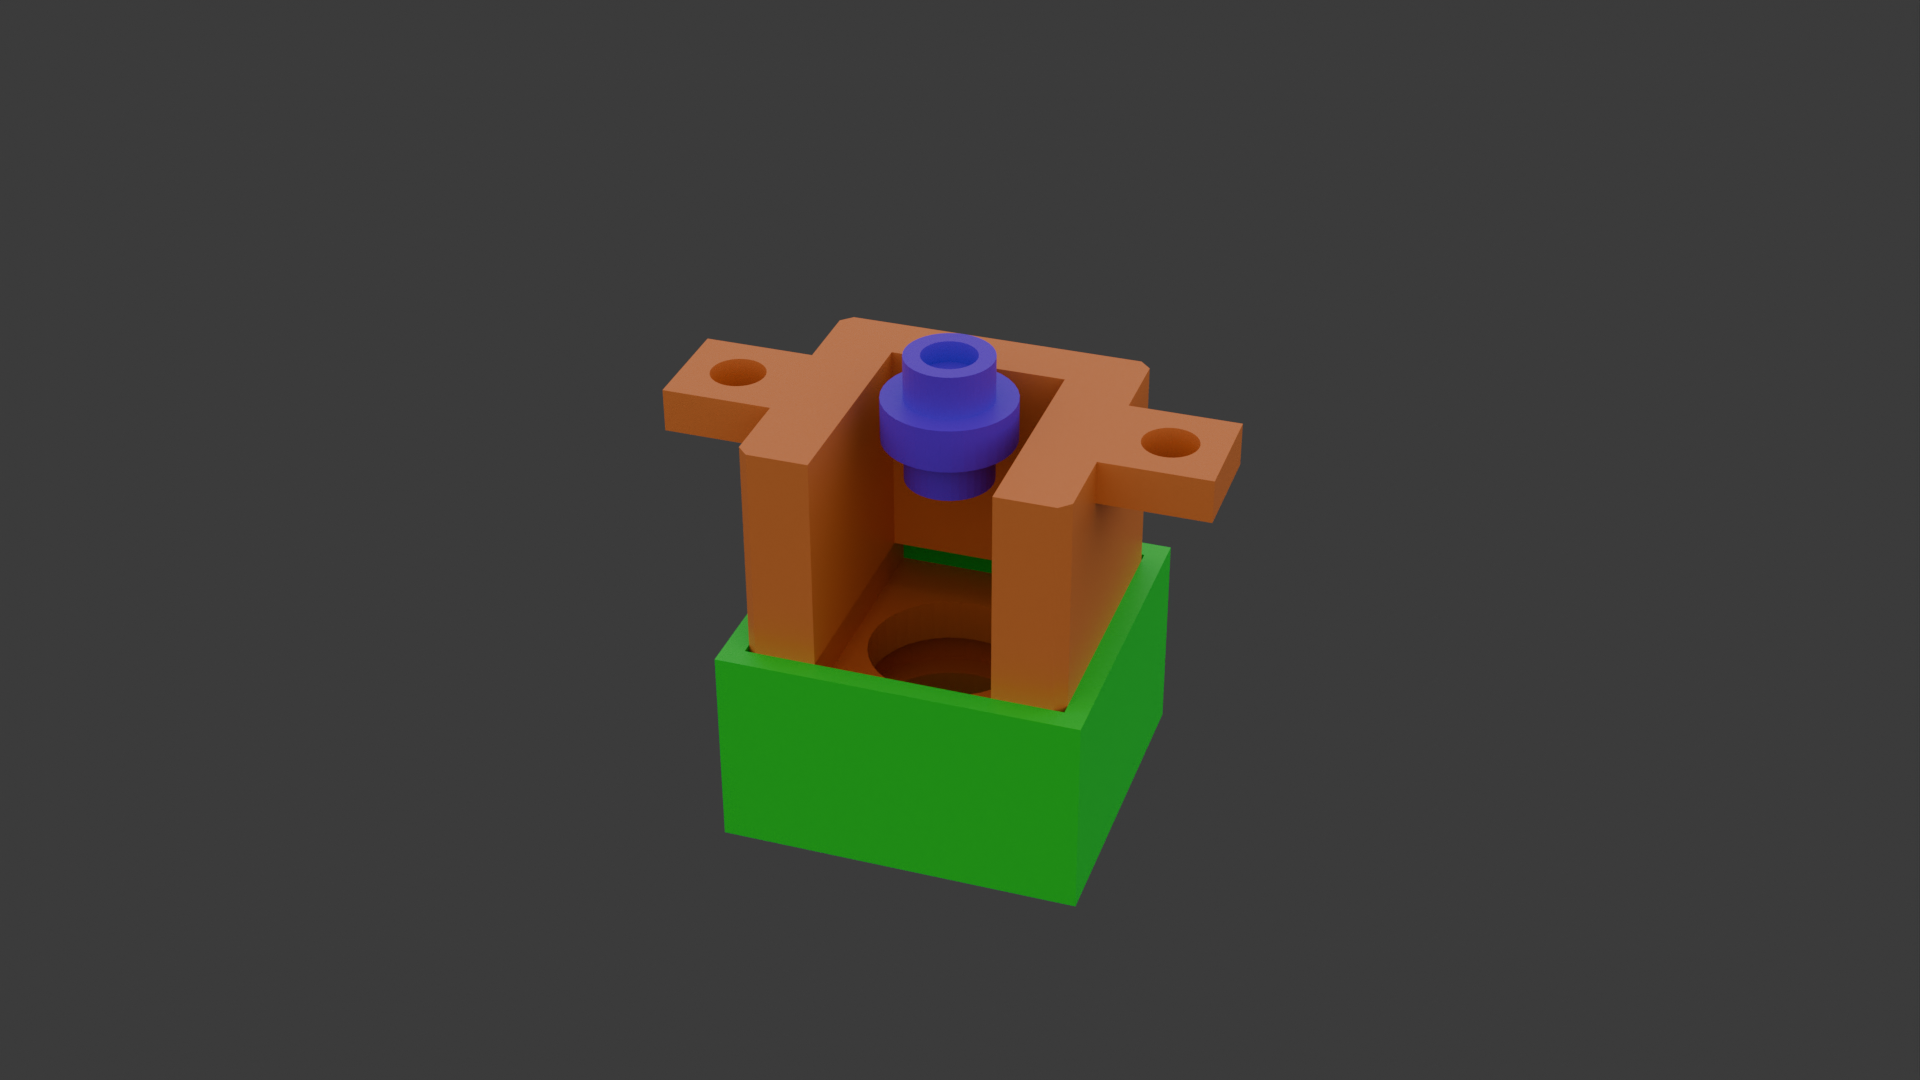
\includegraphics[width=0.875\linewidth]{d_a.png} % Replace with your image file name
    \caption{Caption for the image}
\end{figure}

% \clearpage

\begin{figure}[p]
    \centering
    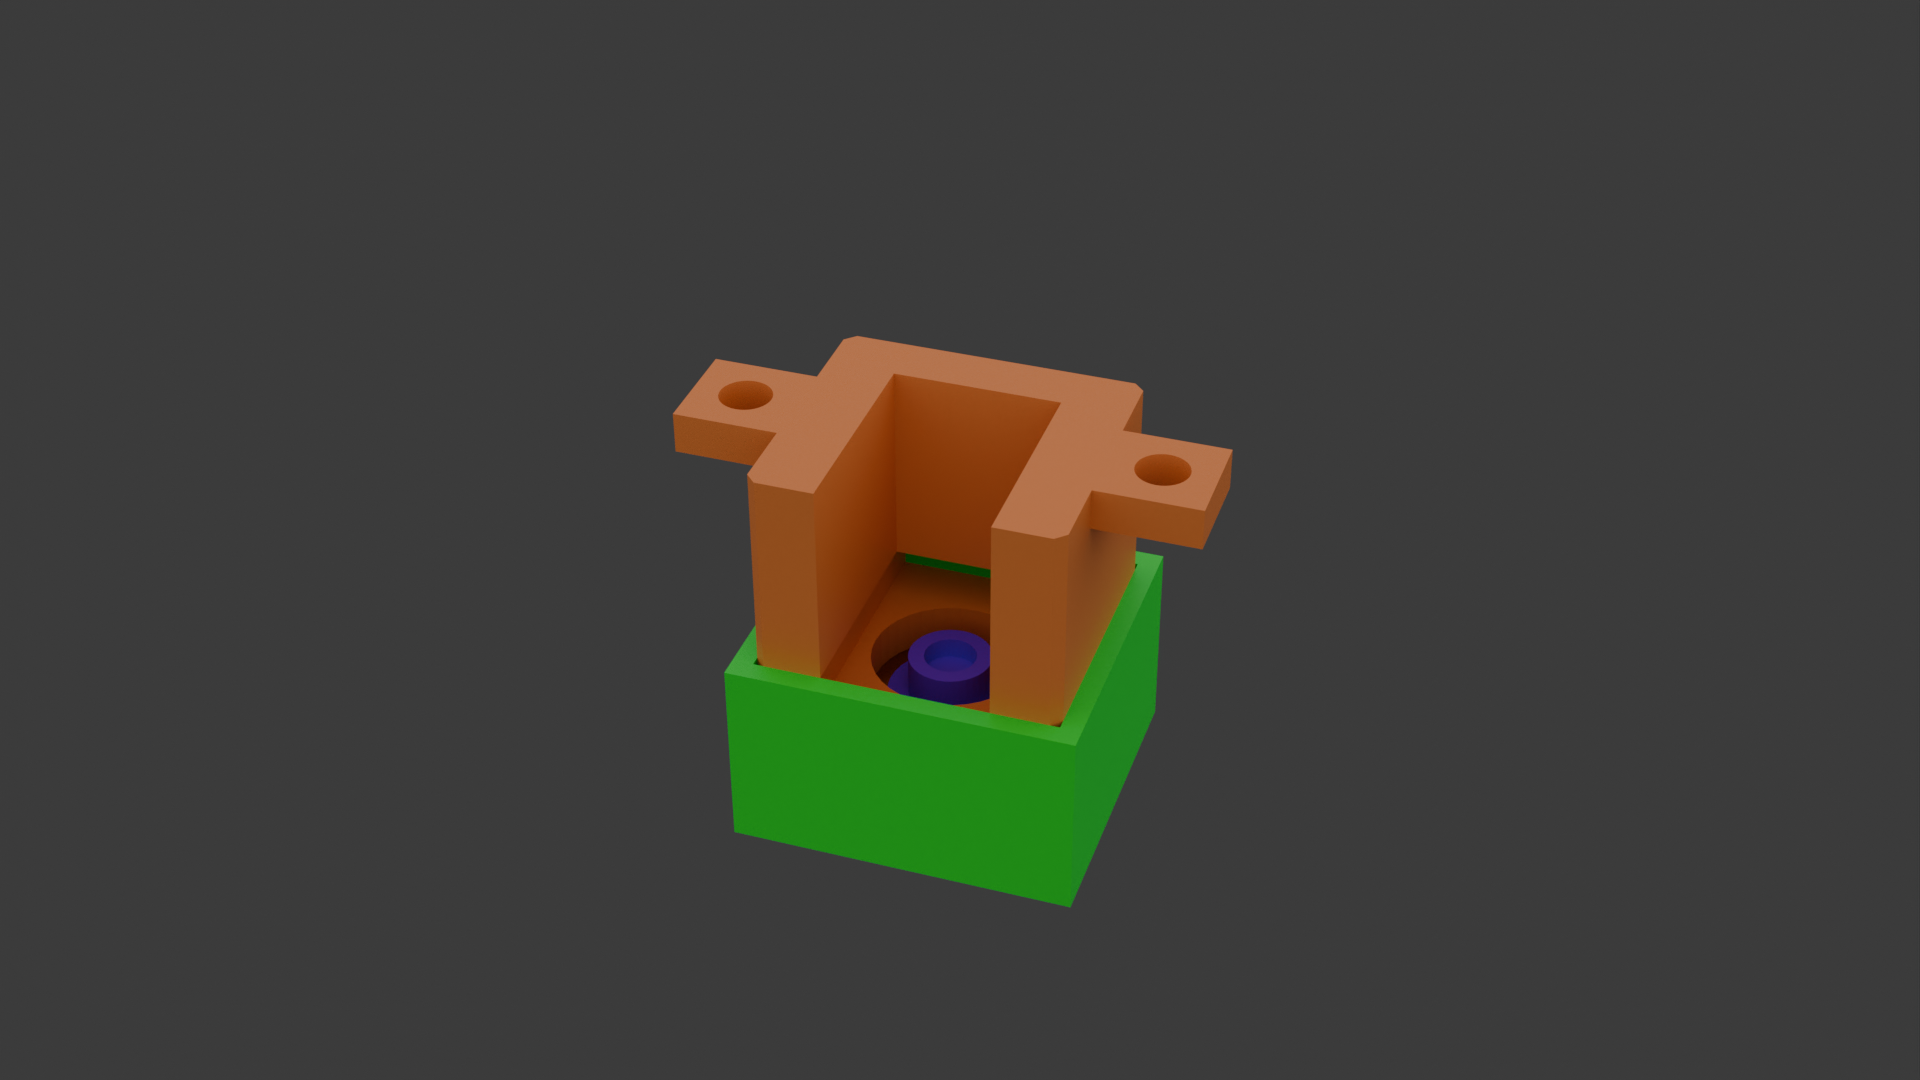
\includegraphics[width=0.875\linewidth]{d_b.png} % Replace with your image file name
    \caption{Caption for the image}
\end{figure}

% \clearpage

\begin{figure}[p]
    \centering
    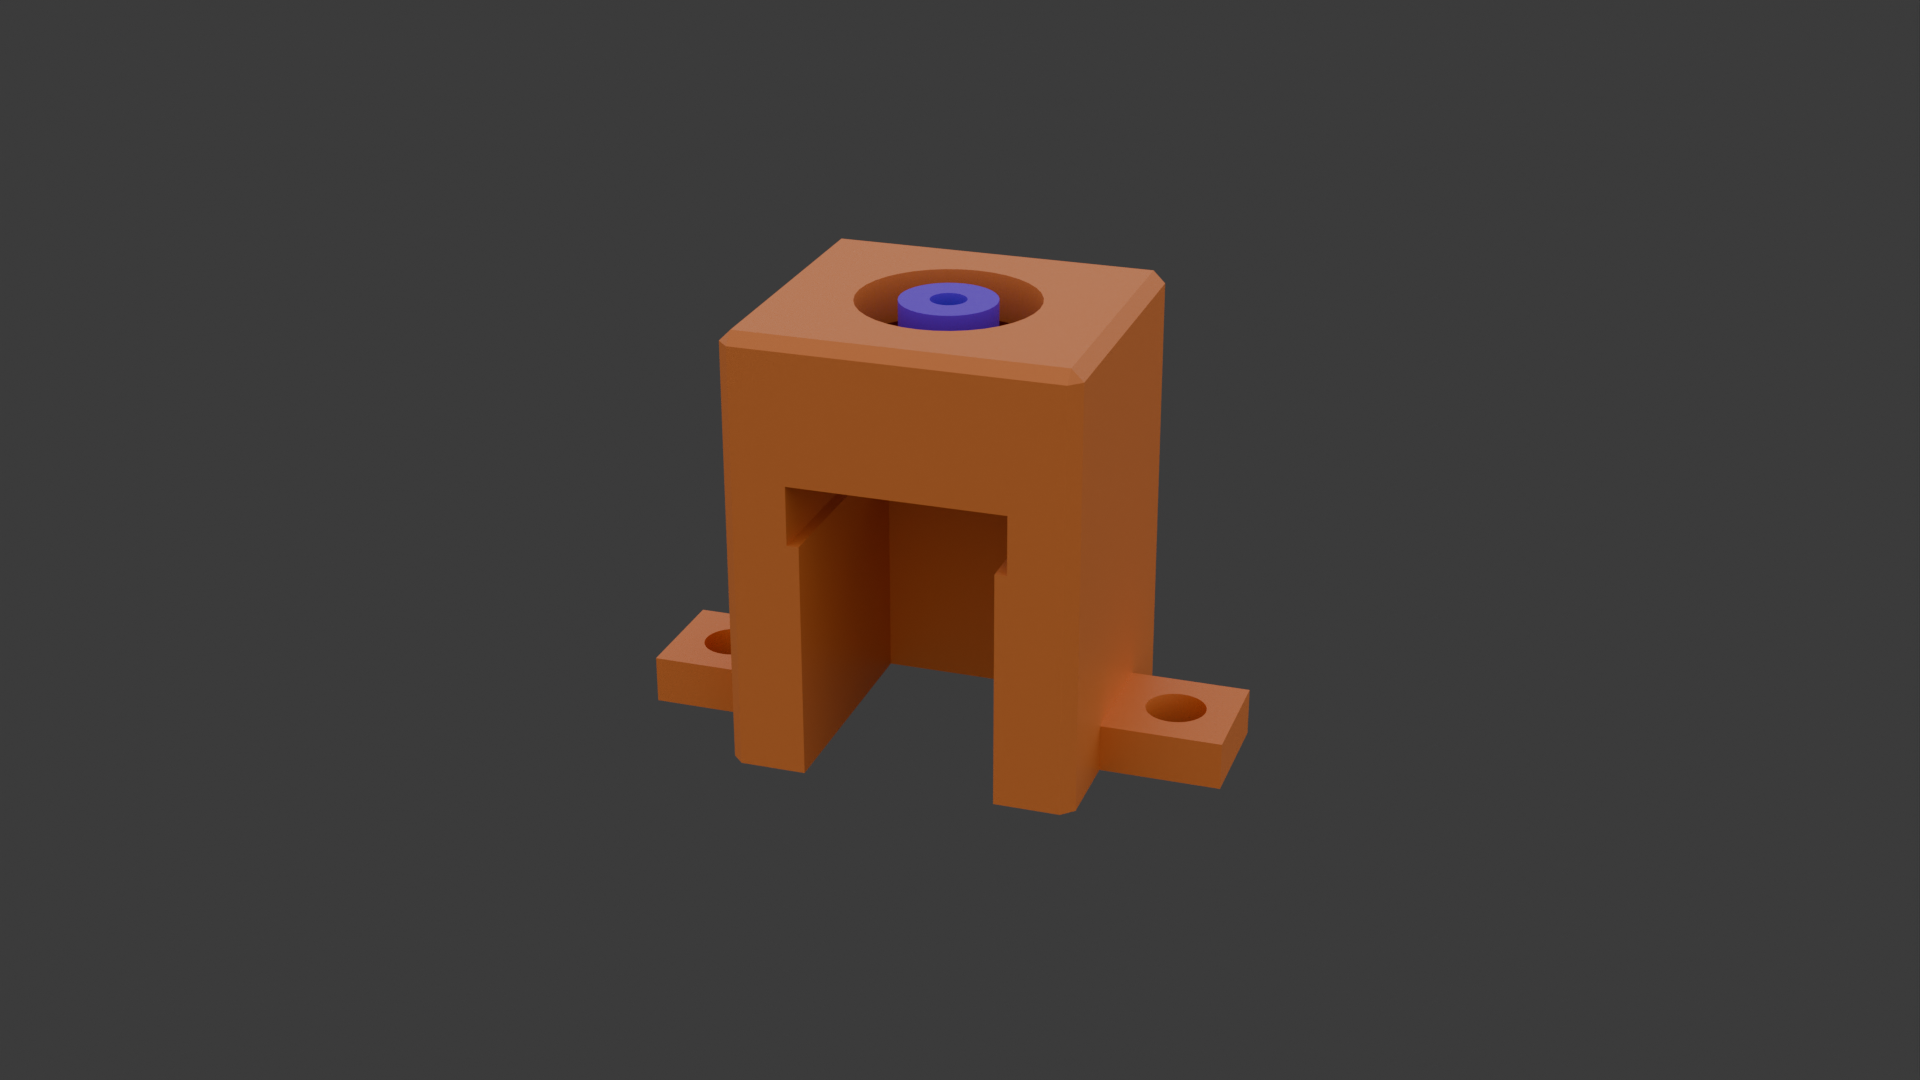
\includegraphics[width=0.875\linewidth]{e.png} % Replace with your image file name
    \caption{Caption for the image}
\end{figure}

% \clearpage

\begin{figure}[p]
    \centering
    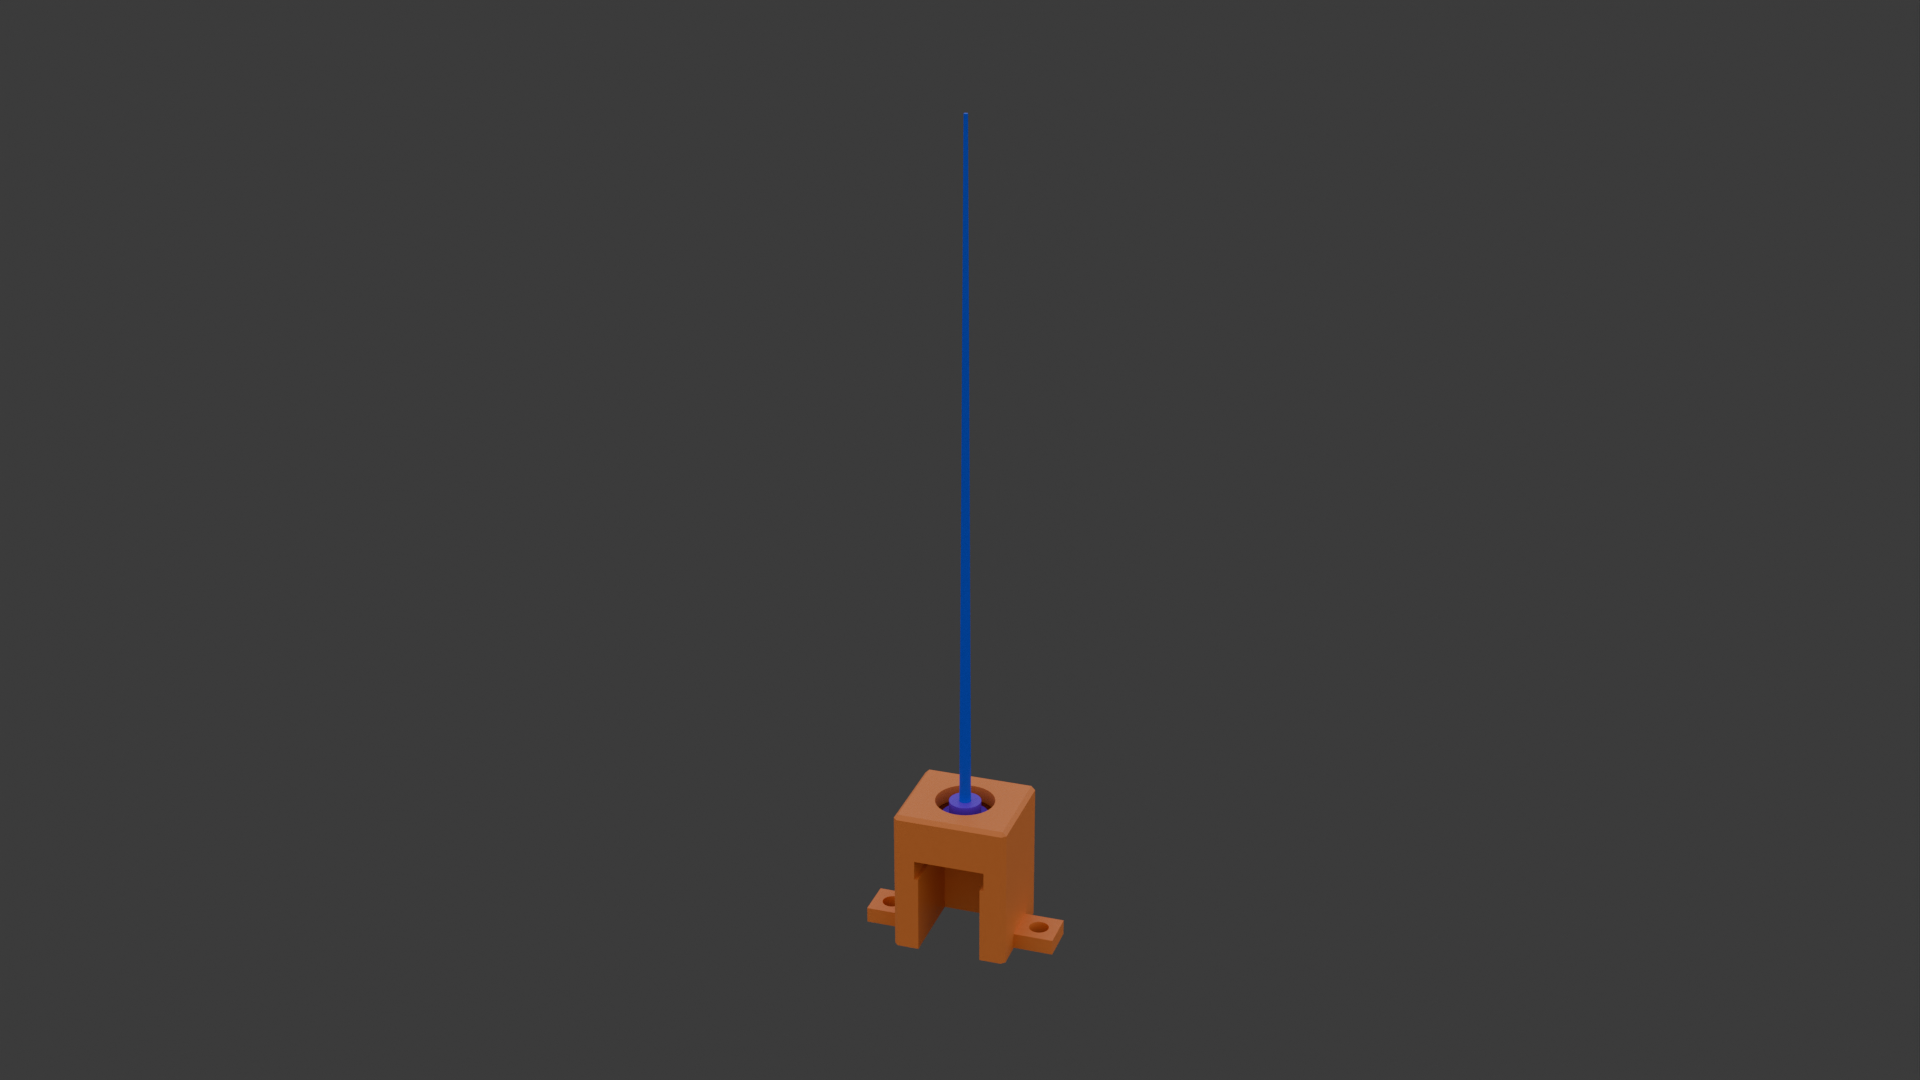
\includegraphics[width=0.875\linewidth]{f.png} % Replace with your image file name
    \caption{Caption for the image}
\end{figure}

% Add more figures and captions as needed

% \end{landscape}


\end{document}
